% \begin{itemize}
%     \item Using the runtime portion of the data you collected during the performance runs, produce a speedup chart showing the scaling performance of your Basic OMP across all levels of concurrency and problem sizes in this assignment. This will be a single chart containing 3 datasets, one for each of p=4,16,64.
%     \item Discuss the performance of your Basic OMP-omp across the set of problem sizes N and concurrency levels P. Describe how speedup changes as a function of problem size, and give an explanation as to why you think that change occurs.
% \end{itemize}

% For the threads = 4 and 16, the speedup shows the steady increase nearing to the ideal speedup of 4 and 16 respectively as the matrix size N increases. According to the Amdahl's law\cite{amdahl1967validity}\footnote{Amdahl's law describes the theoretical maximum speedup that can be achieved in a parallel system based on the portion of a task that must be executed serially. The theoretical speedup limit for a problem size \(n\) and \(p\) parallel processors is given by: \( S(n, p) = \frac{1}{f + \frac{1-f}{p}} \), where \(f\) is the portion of the program that must remain serial, and \((1-f)\) is the parallelizable portion. For smaller values of \(f\), the closer the speedup is to the ideal scaling with \(p\).}, this behavior is expected because for larger matrix sizes, the overhead of the serial portion and the introduction of multithreading should be minimal. 

% For the threads = 64, N = 2048 shows the highest speedup and this is expected, however, N = 512 gives the lower speedup than N = 128 and this is unexpected. We still don't know why this happens.

% \begin{figure}
%     \centering
%     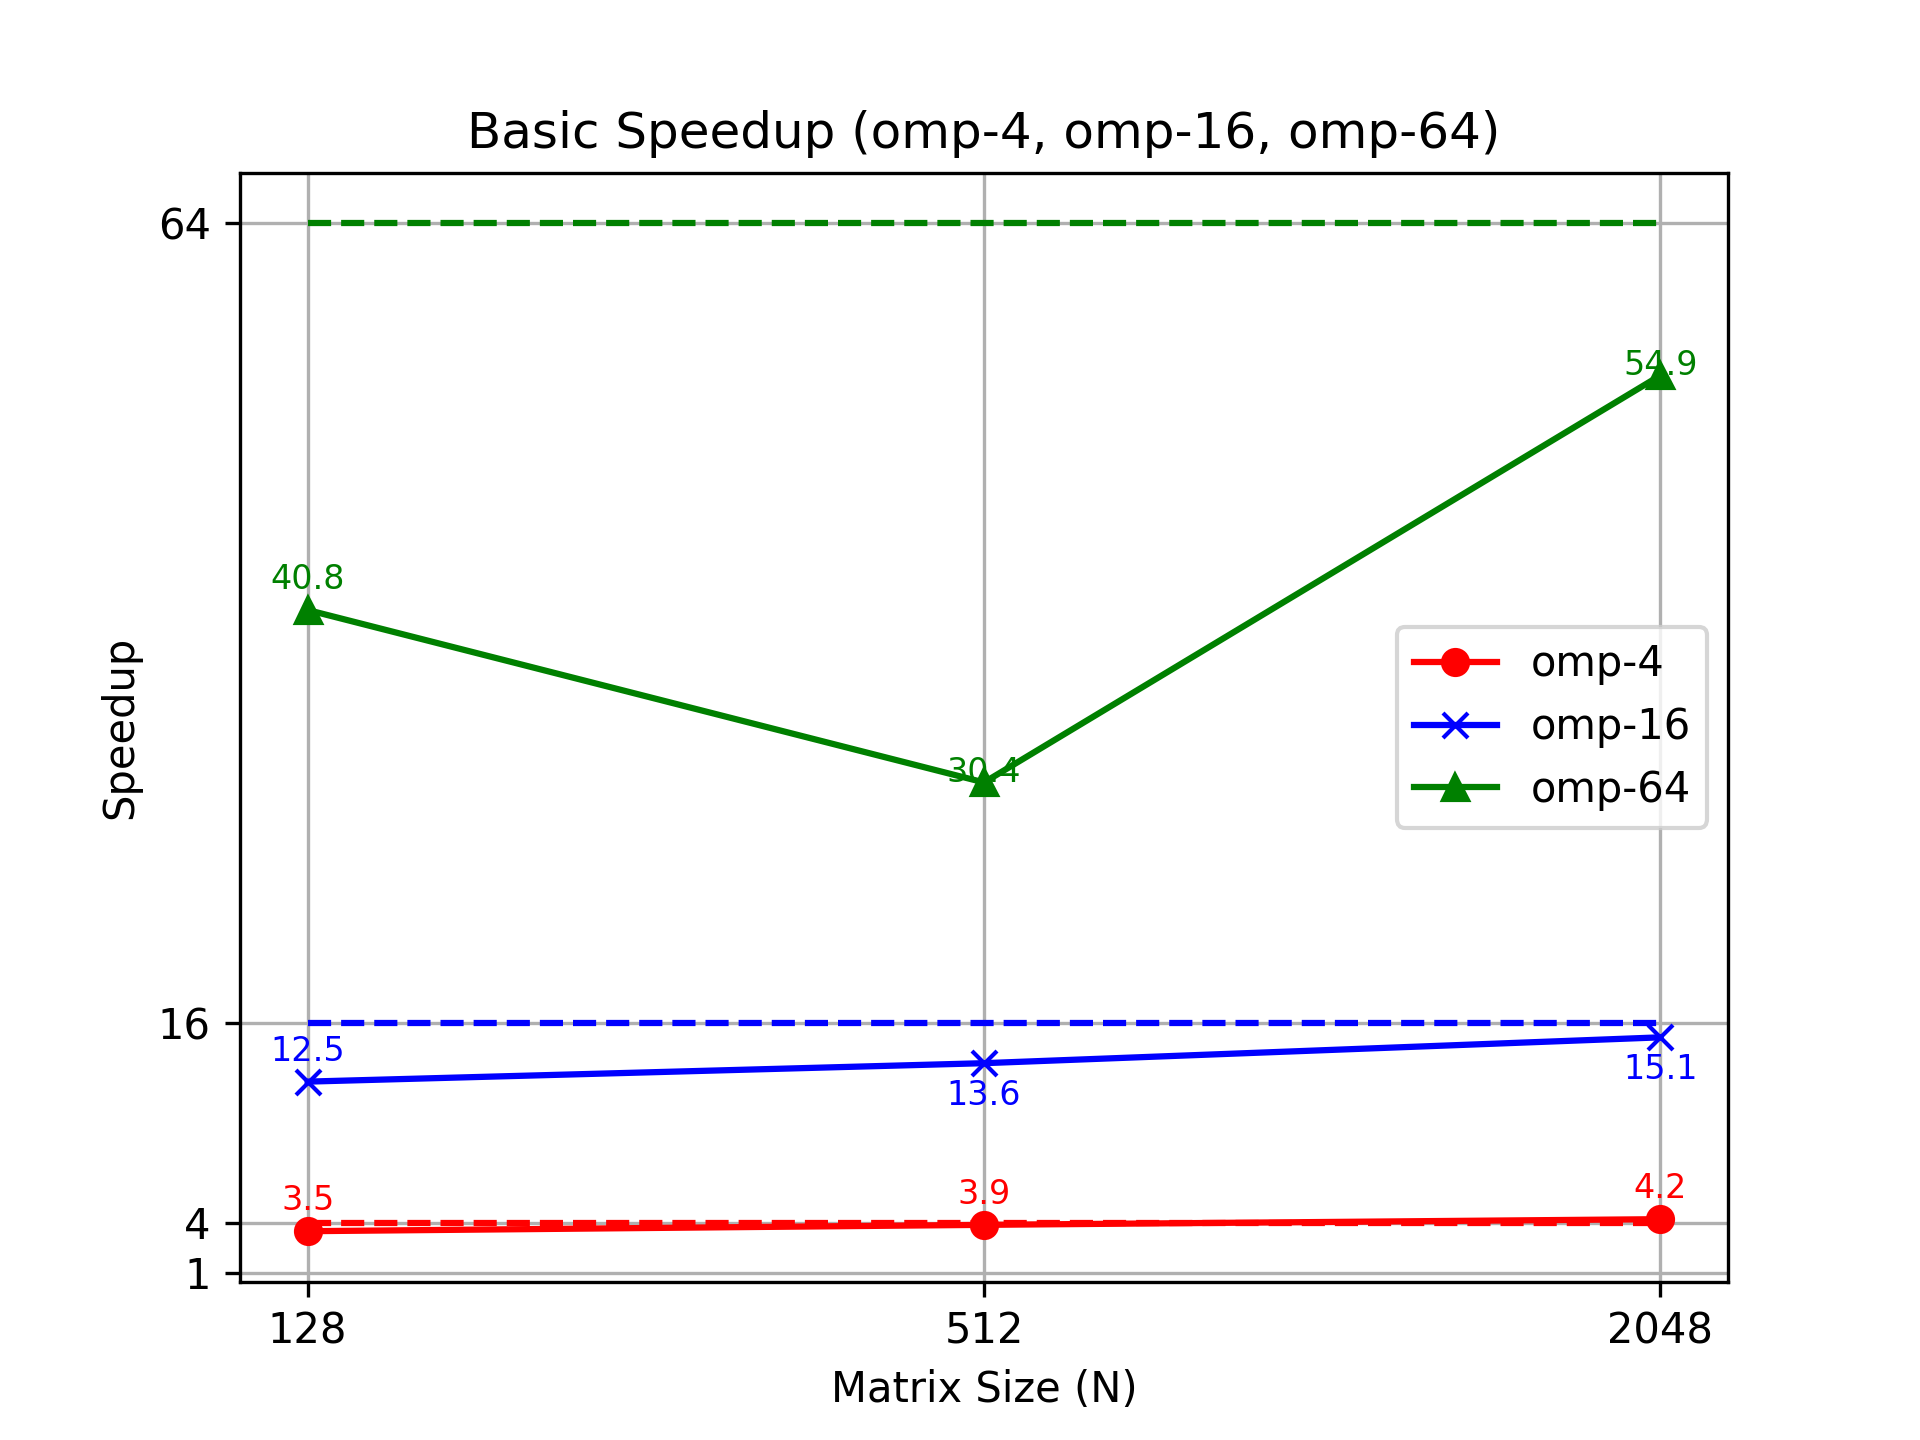
\includegraphics[width=1.0\linewidth]{images/Basic_Speedup.png}
%     \caption{Caption}
%     \label{fig:basic-speedup}
% \end{figure}

The scaling performance of the Basic OMP implementation was analyzed across different concurrency levels (\(p = 4, 16, 64\)) and matrix sizes (\(N = 128, 512, 2048\)). Figure~\ref{fig:basic-speedup} shows the speedup chart, illustrating the relationship between concurrency levels and problem sizes, allowing us to evaluate the efficiency of the parallelization approach.

For thread counts of 4 and 16, the speedup demonstrated a steady increase as the matrix size \(N\) increased, approaching the theoretical ideal speedup of 4 and 16, respectively. This behavior aligns well with expectations based on Amdahl's Law \cite{amdahl1967validity}, which suggests that for larger problem sizes, the impact of the serial portion of the code becomes less significant, thereby reducing overhead and enhancing the effectiveness of parallel execution. In other words, larger matrix sizes increase the computational workload sufficiently to minimize the negative impact of serial portions, thus leading to near-ideal speedup values.

For a thread count of 64, the results were somewhat mixed. The highest speedup was observed for \(N = 2048\), which was expected given the increased computational workload and better utilization of the available cores. However, an unexpected observation was made for \(N = 512\), where the speedup was lower compared to \(N = 128\). This deviation requires further investigation.

\begin{figure}[htbp]
    \centering
    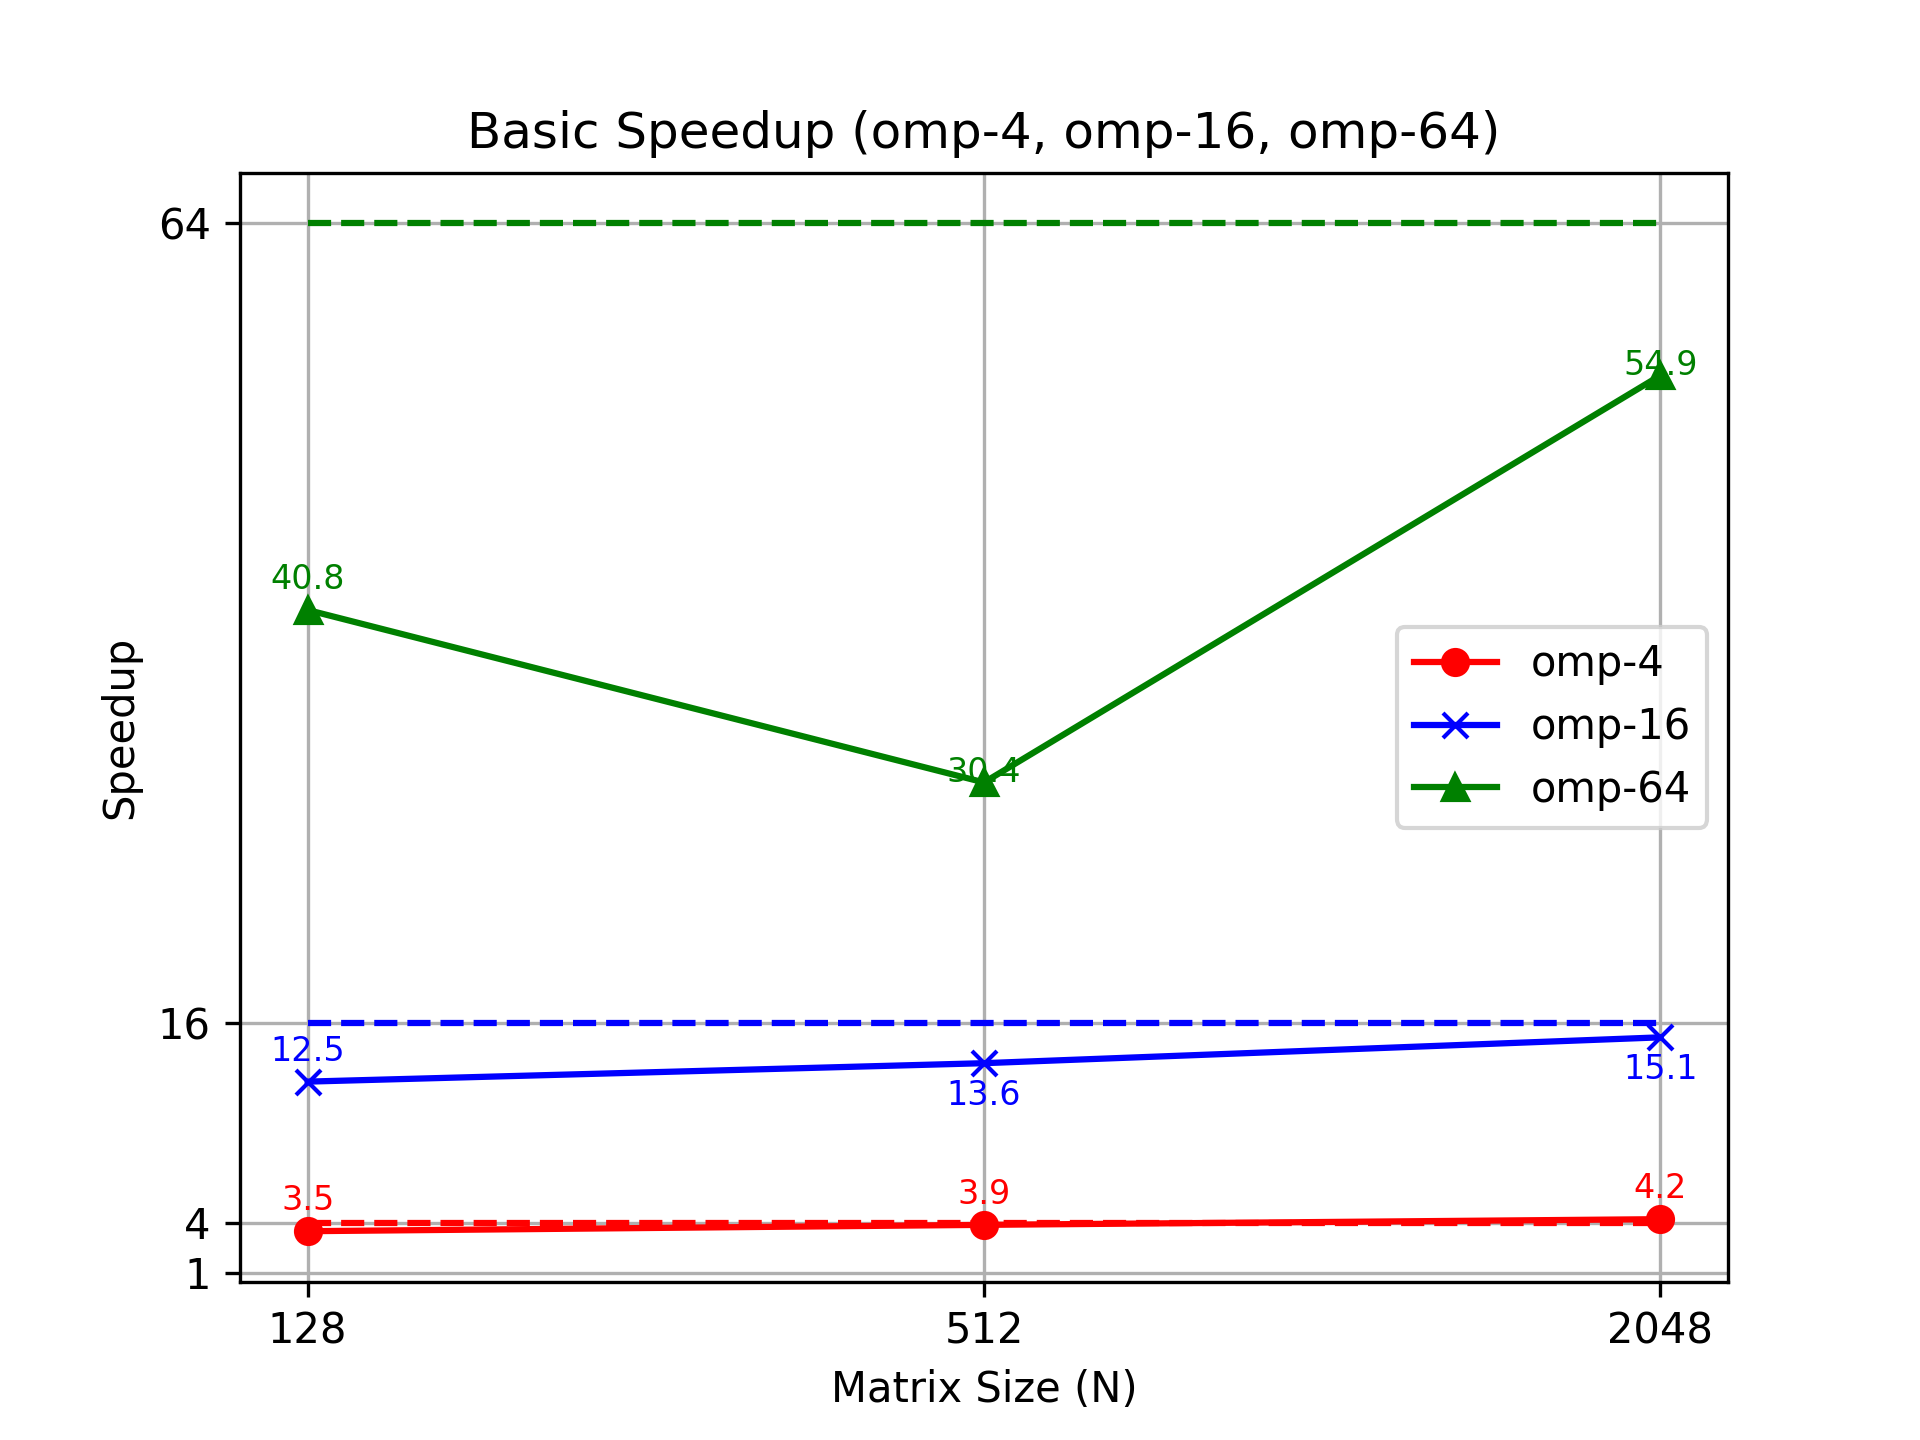
\includegraphics[width=1.0\linewidth]{images/Basic_Speedup.png}
    \caption{\textbf{Speedup of Basic OMP with OpenMP Parallelization.} The figure shows the speedup achieved by the Basic OMP implementation at different concurrency levels (\(p = 4, 16, 64\)) for matrix sizes of \(N = 128, 512, 2048\). The ideal speedup for each concurrency level is also shown for comparison, highlighting the efficiency of parallelization as the matrix size increases. It is observed that for \(p = 64\), the speedup for \(N = 512\) is unexpectedly lower compared to \(N = 128\), suggesting potential issues such as cache contention or memory bandwidth limitations.}
    \label{fig:basic-speedup}
\end{figure}

Interestingly, when measuring runtime using \texttt{std::chrono::high\_resolution\_clock}, as shown in Figure~\ref{fig:basic-speedup-chrono}, the results appear more consistent with the expected outcomes of Amdahl's Law. Specifically, for each thread count, \(N = 128\) consistently achieves lower speedup, while larger \(N\) values yield speedup results that are closer to the theoretical ideal. This steady increase in speedup as \(N\) increases suggests that the instrumentation code used in Listing~\ref{listing:measuring-elapsed-time} provides a more accurate representation of the expected scaling behavior.

\begin{figure}[htbp]
    \centering
    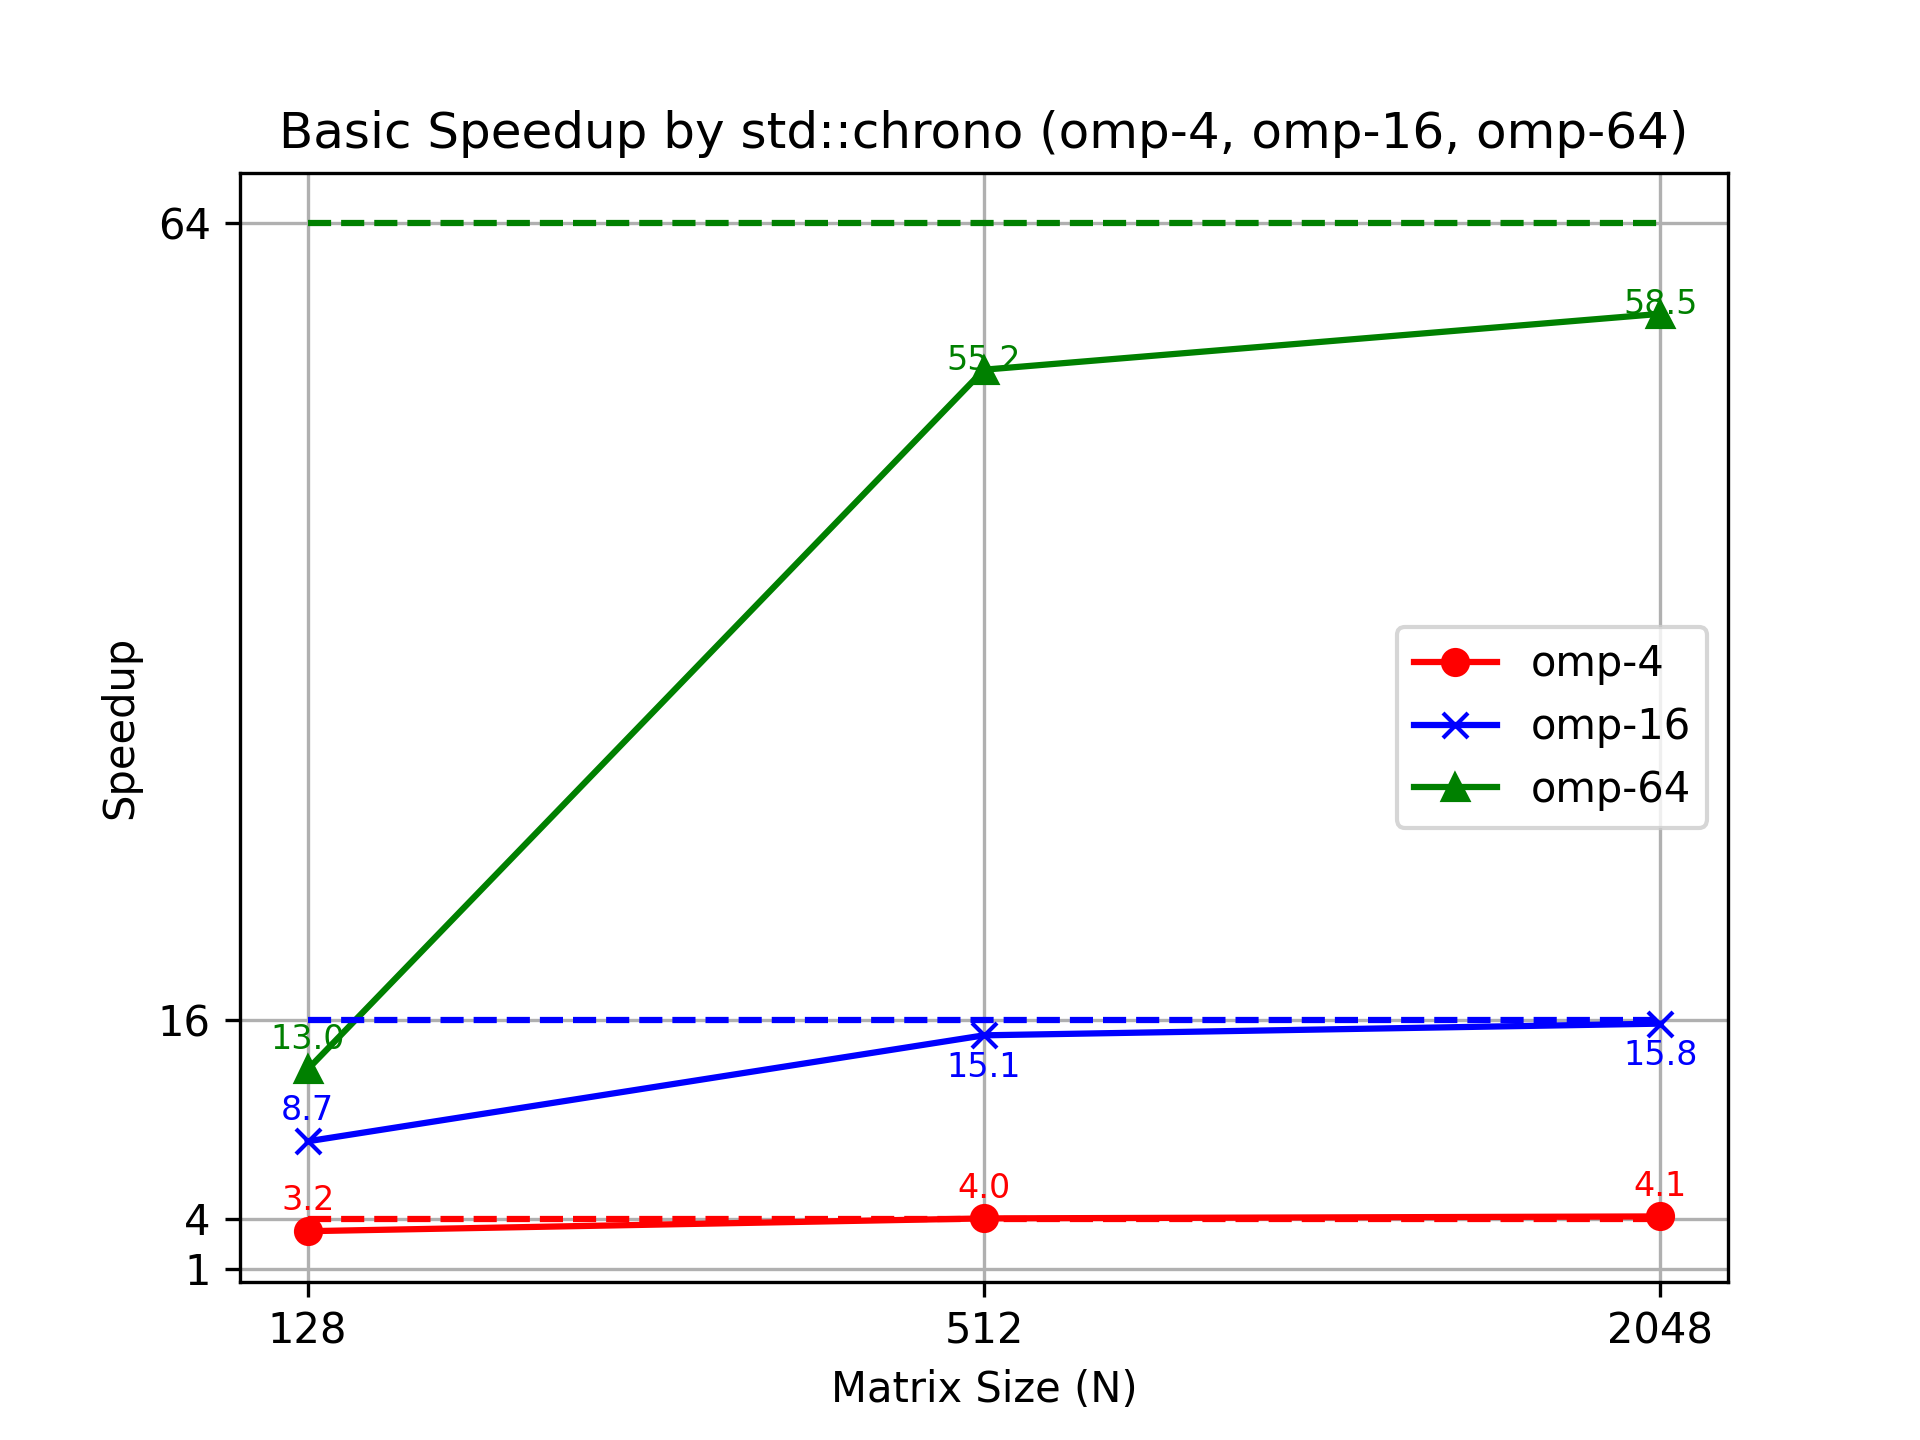
\includegraphics[width=1.0\linewidth]{images/Basic_Speedup_chrono.png}
    \caption{\textbf{Speedup of Basic OMP with OpenMP Parallelization measured by std::chrono::high\_resolution\_clock.} This figure shows the speedup results when using \texttt{std::chrono::high\_resolution\_clock} for measuring elapsed time. Unlike the previous measurements, the speedup values exhibit more predictable scaling behavior, consistent with Amdahl's Law, where larger matrix sizes (\(N = 512\), \(N = 2048\)) result in improved speedup, while \(N = 128\) demonstrates lower efficiency.}
    \label{fig:basic-speedup-chrono}
\end{figure}

\begin{lstlisting}[caption={Instrumentation code for measuring the elapsed time of MM},label={listing:measuring-elapsed-time},name=measuring-elapsed-time,float=htbp,style=mystyle,language=C++]
setup(n, A, B, C);
start_time = get_high_resolution_clock_now();
square_dgemm(n, A, B, C);
end_time = get_high_resolution_clock_now();
elapsed_time = end_time - start_time;
\end{lstlisting}